%% USPSC-Cap2-Desenvolvimento.tex 

% ---
% Este capítulo, utilizado por diferentes exemplos do abnTeX2, ilustra o uso de
% comandos do abnTeX2 e de LaTeX.
% ---

\chapter{Desenvolvimento}\label{cap_exemplos}

\section{Revisão sistemática}
O estudo de Revisão Sistemática da Literatura seguiu as recomendações Preferred Reporting Items for Systematic Reviews and Meta-Analisys – PRISMA.
Foram buscados os termos: “patent mining”, “patent”, “random forest”, “machine learning” - nas seguintes bases de dados: Periodicos CAPES, Microsoft research, Semantic Scholar e Google Scholar. O intervalo de publicação dos artigos selecionados estão entre 2012 a 2020 e restrito a somente artigos escritos em inglês.

\subsection{Descrição do objeto de estudo}
Foi realizado a extração de dados de documentos de patentes no site Free Patents Online - FPO (https://www.freepatentsonline.com/). Este site contem os dados dos documentos de patentes de forma pública.

\subsection{Delineamento da pequisa}
Foi buscado o termo “agronomy” e filtrado para somente documentos de patentes registrados nos Estados Unidos. Foi totalizado 12906 patentes, dos quais selecionamos uma amostragem das 200 primeiras patentes. Construímos uma aplicação de webscraping na linguagem Python para realizar a extração dos dados de documentos de patentes.  Os dados extraídos foram armazenados em um banco de dados.

\section{Materiais e métodos}

\subsubsection{Extração dos dados}
A aplicação de webscraping dos dados de documentos de patentes foi escrita na linguagem de programação Python, com uso das bibliotecas \textit{requests} e \textit{BeautifulSoup}. Essa aplicação é modular o suficiente para que seja definido quantos documentos de patentes terão suas informações extraídas, como também quais informações serão extraídas, como demonstrado na figura \ref{webscraping_flow_image}. Os dados são organizados na forma de tabela e armazenado em um pequeno banco de dados feito em \textit{SQLite}.

\begin{figure}[ht!]
	\centering
	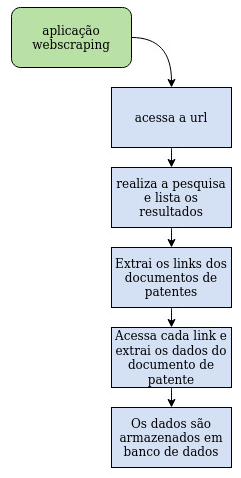
\includegraphics[scale=0.5]{imagens/tcc_webscraping.jpg}
	\caption{Fluxo de captura dos dados de documentos de patente 
			 \label{webscraping_flow_image}}
\end{figure}


\subsubsection{Construção do dicionario}
A construção do dicionario que será utilizado no projeto é composto pelas seguintes etapas, figura \ref{dicionario_flow_image}, geração de um corpora de documentos de patentes, pre processamento do corpora, obtenção da matriz de documento-termo (Document-Term Matrix – DTM) e aplicação do modelo Latent Dirichlet allocation (LDA). A partir dos tópicos apresentados pelo resultado do LDA, são adicionados ao tópicos, palavras relacionadas, tais como sinônimos, hiperônimos e hipônimos através do banco de dados wordnet.

\begin{figure}[ht!]
	\centering
	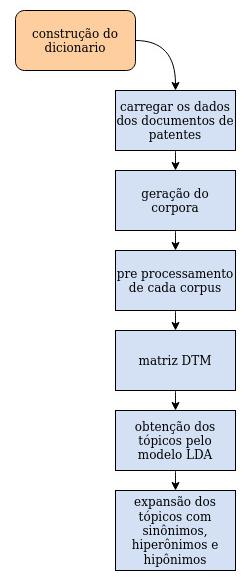
\includegraphics[scale=0.5]{imagens/tcc_dicionario.jpg}
	\caption{Fluxo de criação do dicionario
			 \label{dicionario_flow_image}}
\end{figure}

\subsection{Validação do dicionario}
A avaliação do dicionario obtido, consiste em observar se o valor k utilizado para geração de tópicos conseguiu separar adequadamente os assuntos contidos no corpora.

\subsection{Classificação a partir do dicionario}
Esta etapa consiste em utilizar o dicionario para classificar os documentos de patentes a partir da iteração com cada termo do dicionario para o conjunto de termos de cada documento, classificando para cada tópico. Esta tarefa é demorada e o tempo necessário aumenta exponencialmente conforme aumenta o tamanho do corpora utilizado. A base de dados gerada será usada para ensinar ao modelo como classificar novos documentos de patentes.


\subsection{Modelagem}
Utilizaremos três dos modelos mais citados na classificação de texto, o RandomForest, Naive Bayes e SVM para avaliar qual se adéqua melhor a essa classificação. Usaremos as técnicas de pré processamento para garantir que o mesmo dado será testado igualmente para cada modelo e escolheremos o modelo de melhor acurácia como modelo final.


\section{Resultados}

\subsection{Extração de dados}

Extraímos uma amostra no total de 904 documentos de patentes através do uso da técnica de webscraping. Destes documentos, os dados de \textbf{Titulo} e \textbf{Resumo} foram pré processados, removendo as quebras de linhas, espaços no inicio e fim da frase, uso de somente um espaço como separador e transformação do texto em minúsculo. Estes dados foram concatenados e usados para a montagem do corpora de documentos de patentes, que poderá ser utilizado para outros projetos. Podemos visualizar na figura \ref{wordcloud_pre_image} como é distribuida a relação de palavras.

\begin{figure}[ht!]
	\centering
	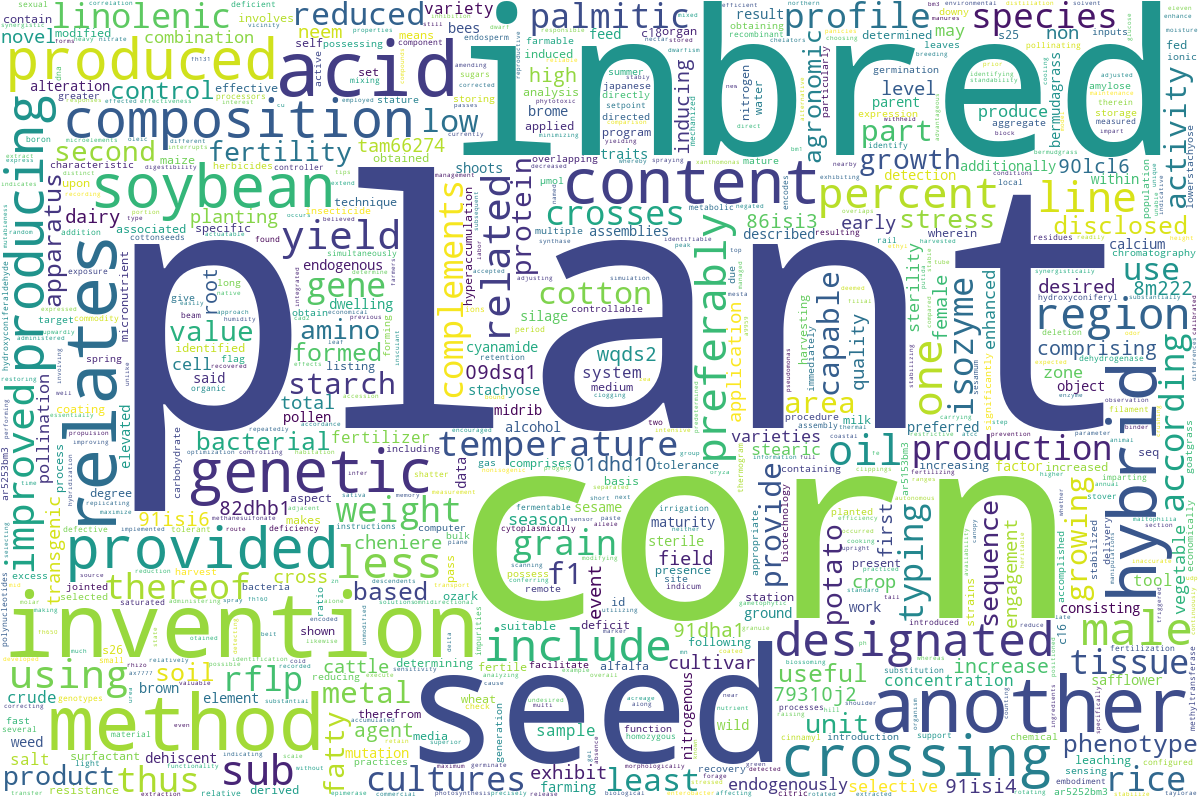
\includegraphics[scale=0.3]{imagens/wordcloud_preprocess.png}
	\caption{Construção nuvem de palavras dos termos mais representativos para este corpora.
			 \label{wordcloud_pre_image}}
\end{figure}

\subsection{Construção do dicionario}

A construção do dicionário engloba o levantamento de tópicos, validação dos tópicos e a expansão do dicionário.

\subsubsection{Levantamento de tópicos}

Foi utilizado o corpora de documentos de patentes feito no passo anterior, onde foi removido as \textbf{stopwords} (palavras que não possuem importância a frase, por exemplo em Inglês: The, from, a, an, with, etc.), foram removidos também caracteres numéricos e especiais. O conteúdo de cada corpus foram separados em uma lista palavras, este processo denomina-se como geração de \textbf{tokens} e cada token foi desflexionado para a sua palavra raiz (\textbf{lemmas}). Obtivemos 904 conjuntos de palavras normalizadas, representando cada documento de patente e que esta pronto para ser utilizado em modelos de Processamento de Linguagem Natural e em modelos de Aprendizado de Maquina.
Aplicamos o \textbf{modelo LDA}, com os seguintes parâmetros - random\_state igual a 100, update\_every igual a 1, chuncksize igual a 100, passes igual a 10 e alpha automático. Para definir a quantidade de tópicos k, usamos um laço de 40 interações e anotamos o valor da métrica Coherence.

\begin{figure}[ht!]
	\centering
	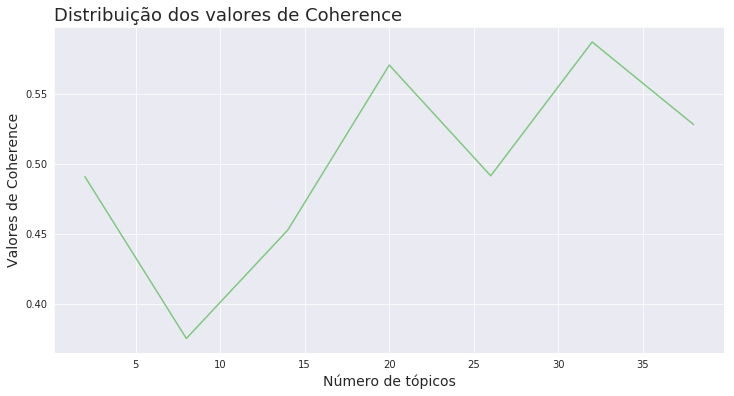
\includegraphics[scale=0.6]{imagens/distr_dos_valores_de_coherence.png}
	\caption{A distribuição dos valores de Coherence ao longo da variação do \textbf{parâmetro k}, permite que observemos qual a quantidade de tópicos mais relevantes a se utilizar.
			 \label{dist_coherence_image}}
\end{figure}

O gráfico da figura \ref{dist_coherence_image} aponta que um k igual a 25 resulta no mais alto valor de Coherence. Utilizaremos este valor para k para se definir os títulos de tópico.

\subsubsection{Validação dos tópicos}

Examinamos o tópicos obtidos através da ferramenta pyLDAvis, figura \ref{pyLDAvis_image}. Os termos que compõe os tópicos gerados  representam bem o corpora usado. Temos pouca sobreposição, com exceção do tópico 18, e os termos de cada tópico possuem uma alta relevância com o tema agronomia.  

\begin{figure}[ht!]
	\centering
	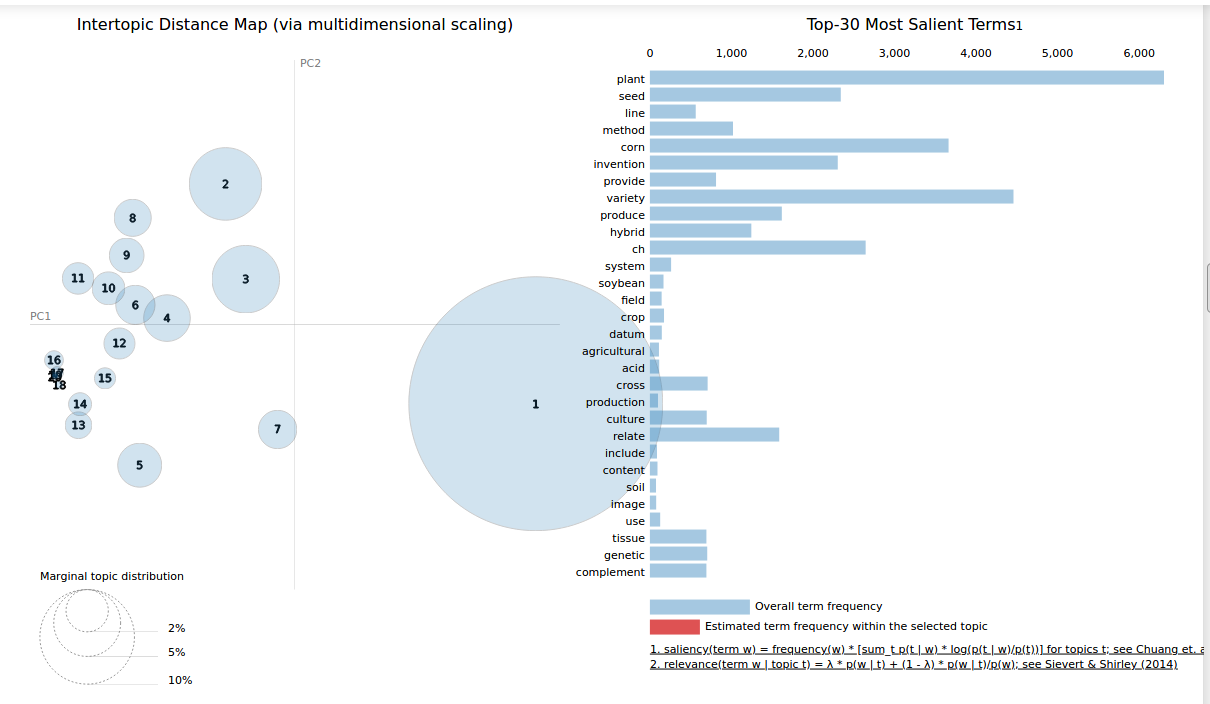
\includegraphics[scale=0.4]{imagens/construcao_dicionario.png}
	\caption{O grafico de bolhas, cada bolha representa um tópico, o tamanho da bolha representa a prevalencia do tópico e a sobreposição de bolhas aponta a similaridade entre os tópicos. O gráfico da direita, as barras representam a relevância do termo para o tópico observado.
			 \label{pyLDAvis_image}}
\end{figure}

\subsubsection{Expansão do dicionário}

Antes de expandir o dicionário, realizamos a remoção dois tópicos que estavam muito similares. Os tópicos geraram no total de 144 termos únicos que foram submetidas ao wordnet e adicionado os sinônimos, hiperônimos e hipônimos destes termos, totalizando 616 termos que representam cada tópico. A estrutura do dicionário criado é composta por três colunas, a primeira é o tópico, a segunda são os termos que estão atrelada ao tópico e a terceira coluna são as palavras derivadas dos termos.

Obtivemos no final um dicionário com com 901 linhas e três colunas, que foi utilizado para fazer uma classificação inicial dos documentos de patentes. 

\subsubsection{Construção da base de dados}

A base de dados composta a partir das informações de identificação documento de patente, o título do documento de patente e o seu resumo. A partir do dicionario fizemos uma classificação, onde atribuímos a cada documento de patente os tópicos a que se referem. A estrutura da base de dados é de 817 linhas e 7 colunas, sendo que 87 linhas foram removidas por não conterem título ou resumo.

\subsubsection{Construção do modelo}

Para a construção do modelo principal, os seguintes modelos foram testados, Random Forest, Naive Bayes e SVM, os principais modelos aplicados em classificação de texto. O seguinte fluxo de analise de dados foi aplicado:

\paragraph{Pre processamento}

\subparagraph{Matriz documento-termo}

Conversão da tabela de entrada em uma matriz documento-termo, esta matriz tem a estrutura da seguinte forma:

\begin{itemize}
  \item colunas: palavras de relevância
  \item linhas: documentos
  \item valores: correspondem ao valor de TF-IDF obtido, quando a palavra não consta na entrada, o valor será igual a zero.
\end{itemize}

A matriz resultante possui 817 linhas e 3492 colunas.
	
\subparagraph{Remoção de stopwords}

Ao converter a tabela de entrada em uma matriz de documento-termo, as colunas são todas palavras de todos os documentos de patente, fazendo-se necessário a remoção de stop-words, resultando em uma tabela com 817 linhas e 3402 colunas.

\subparagraph{Seleção de características}

A seleção de características tem como objetivo selecionar as colunas que possuam maior relevância a coluna alvo. Utilizamos o método RFE para reduzir o numero de colunas para somente 20. Nossa matriz final possui 817 linhas por 20 colunas.

\subparagraph{Modelo}

Os seguintes parâmetros foram utilizados para cada modelo, seguido do valor de acurácia obtido:
	
\begin{itemize}
  \item RandomForest
  \begin{itemize}
    \item critério de separação: Gini
    \item profundidade máxima: 5
    \item validação cruzada de 10 folds
    \item \textbf{acurácia igual a $0.83$}
  \end{itemize}
  \item NaiveBayes
  \begin{itemize}
    \item foram mantidos o valor padrão para cada parâmetro
    \item \textbf{acurácia igual a $0.80$}
  \end{itemize}
  \item SVM
  \begin{itemize}
    \item custo: 1,5
    \item \textbf{acurácia igual a $0.78$}
  \end{itemize}
\end{itemize}	

\subparagraph{Avaliação de parametros}
	
O modelo escolhido foi o RandomForest por ter o maior valor de acurácia, avaliamos se os parâmetros de profundidade máxima poderia ser melhorado como visto na figura \ref{validation_curve_max_depth_rf}.

\begin{figure}[ht!]
	\centering
	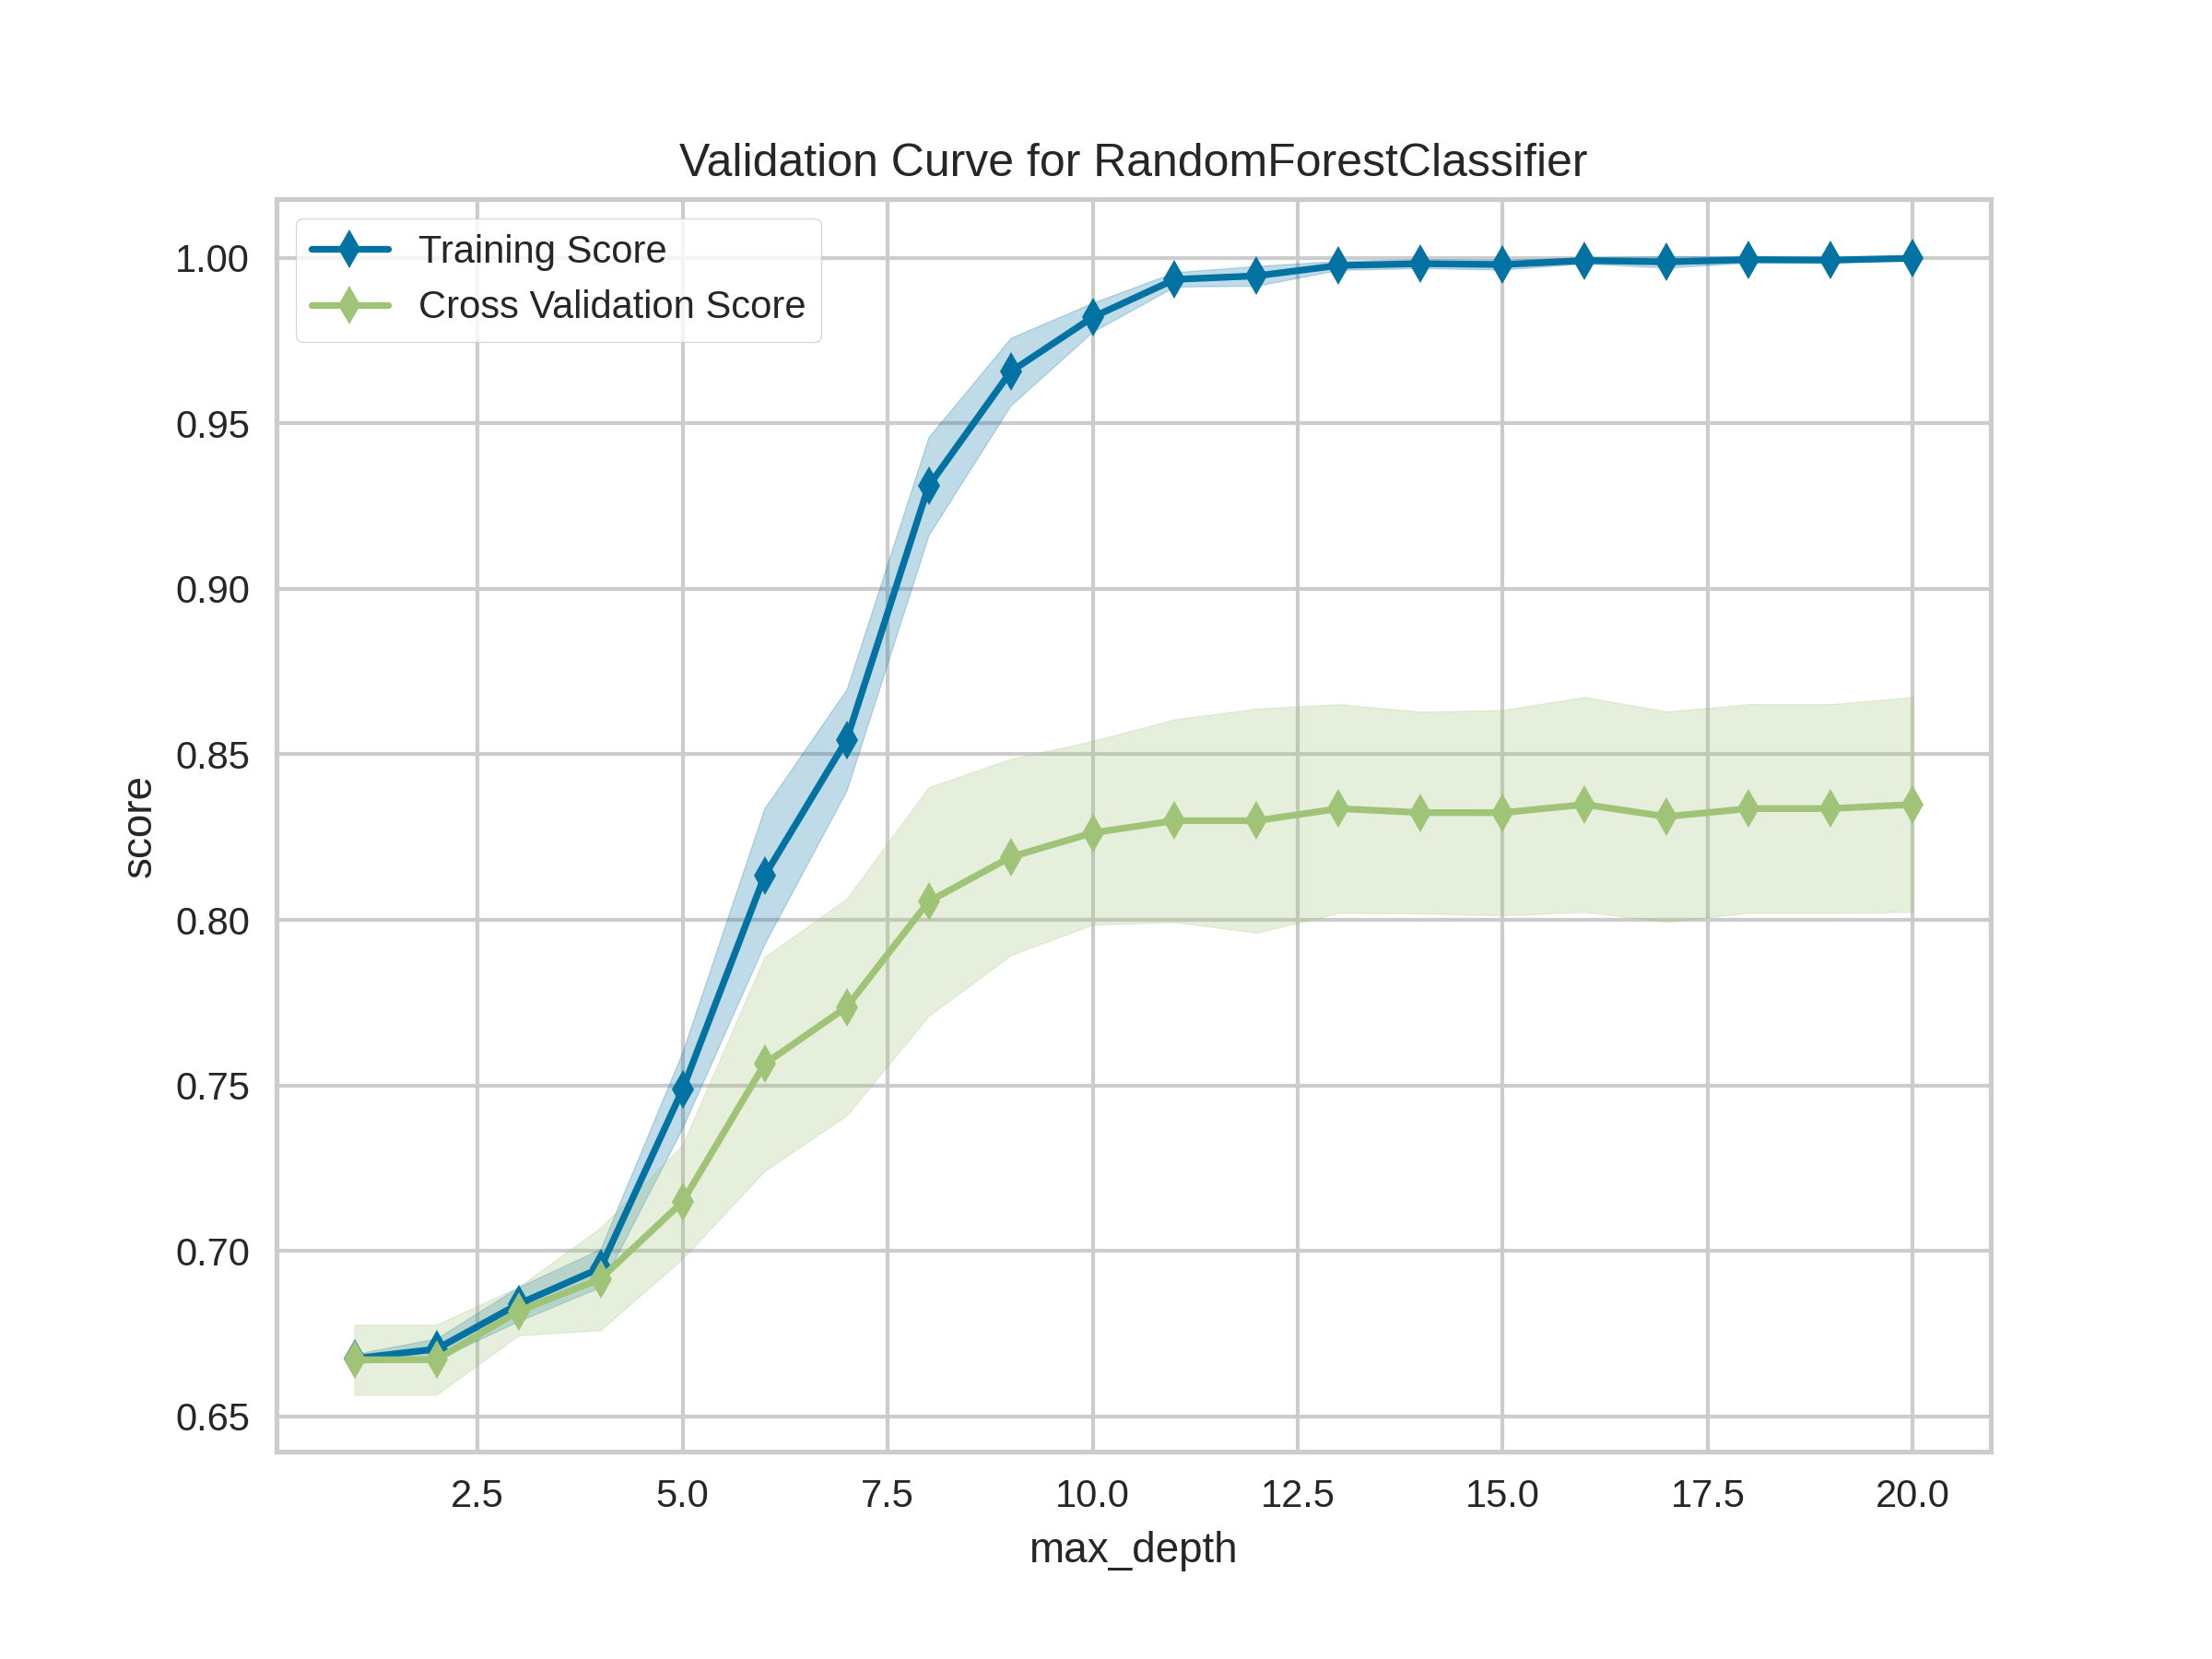
\includegraphics[scale=0.8]{imagens/validation_curve_max_depth_rf.png}
	\caption{Plot do valor de acurácia obtido para cara valor de profundidade máxima. Podemos observar que para os dados de treino e validação se estabiliza após o valor 10.
			 \label{validation_curve_max_depth_rf}}
\end{figure}

Após ajustar o parâmetro de máxima profundidade para 15, obtivemos uma acurácia de 0,84. Não houve um ganho significativo em alterar o parâmetro de máxima profundidade.

\section{Discussão}

Conseguimos realizar a extração bem sucedida de uma amostra de documentos de patentes, do qual pré processamos e criamos um corpora que poderá ser usado não somente para este trabalho como para outros trabalhos com documentos de patentes sobre o tema de agronomia. Fizemos um primeiro levantamento dos tópicos usando o modelo LDA e obtivemos 25 tópicos que serão avaliados e rotulados corretamente. 
Utilizando termos simples para rotular os tópicos neste primeiro momento percebemos que dois tópicos puderam ser removidos por serem semelhantes. Com os termos, expandimos com novos termos que são sinônimos, hiperônimos e hipônimos dos termos associados aos tópicos fazendo com que o nosso dicionário cubra uma área maior do assunto. 
Por fim, testamos três modelos muito utilizados na classificação de textos, o Random Forest, Naive Bayes e SVM. O modelo feito em RandomForest obteve um melhor resultado em comparação aos outros dois modelos, onde o modelo final  alcançou um valor de acurácia de $0.84$, muito mais do que era esperado. 
Acreditamos que aplicando outras técnicas de pre processamento e um teste exaustivo de diferentes valores de parâmetros, há a possibilidade de obter um valor de acurácia acima de $0.90$.

